\section{Frames of reference}
There are different frames of reference, which is defined here. There are the global frame which is the the earth, this frame operates in various coordinate systems such as the \ac{WGS84} and \ac{ECEF}. In addition to this there is a local frame/inerital frame, which is a tangential plane on the surface of the earth int he area the vessel has to operate. Lastly the vessel has a frame attached to this, which is the body frame. All x,y,z frames are righthanded.

Rotation matrices could be of interest here, but see \cite{argo} for now.

\begin{figure}[htbp]
	\centering
	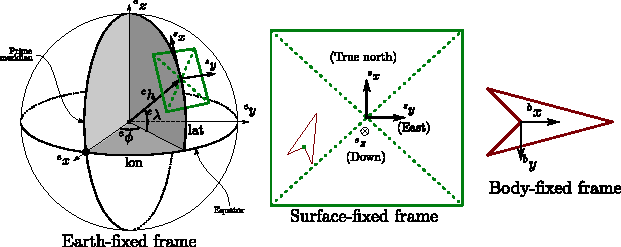
\includegraphics[width=\textwidth]{img/reference_frames}
	\caption{Definitions of the reference frames, using the same system as \cite{argo}.}
	\label{fig:vessel-block-overview}
\end{figure}


\todo[inline]{Note: Theese the x and y variables could be swapped in some of our software, because we started on that earlier than we defined theese frames.}


